%-----------------------------------------------------------------
%	GEOGRAPHIC ANALYSIS
%	!TEX root = ./../main.tex
%-----------------------------------------------------------------
\subsection{Analysis of the path length}
In \Cref{fig:natl-distance-bvln} and \Cref{fig:epac-distance-bvln} we can see the bivariate lognormal distributions of the path length $d$ and lifetime of the storms for the North Atlantic and Northeast Pacific basins separating storms by SST class.

\begin{figure}[H]
	\centering
	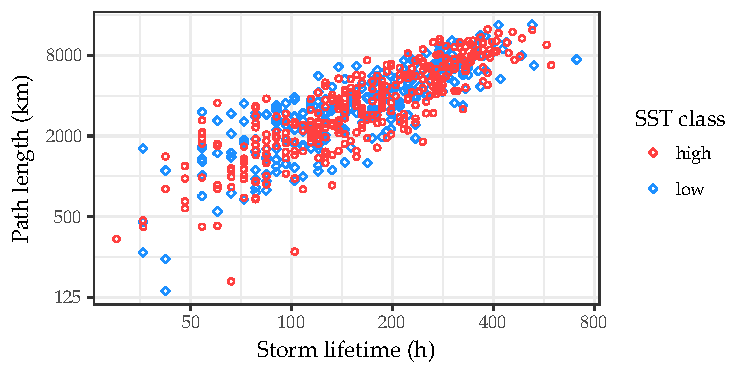
\includegraphics[width=0.8\textwidth]{images/natl-distance-bvln}
	\caption{Bivariate lognormal distribution $f(d, \text{lifetime})$ of the hurricane observations for the North Atlantic basin}
	\label{fig:natl-distance-bvln}
\end{figure}

\begin{figure}[H]
	\centering
	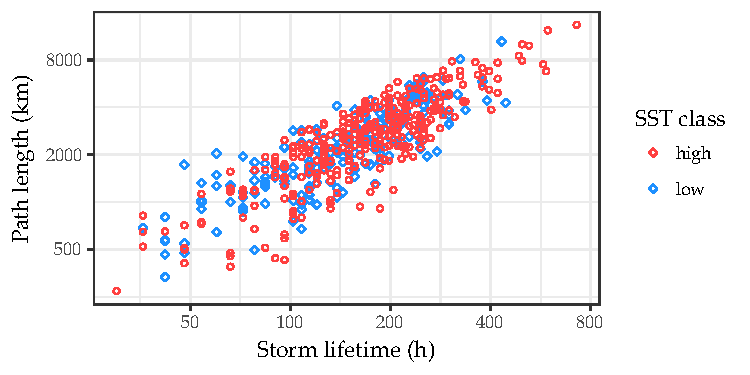
\includegraphics[width=0.9\textwidth]{images/epac-distance-bvln}
	\caption{Bivariate lognormal distribution $f(d, \text{lifetime})$ of the hurricane observations for the Northeast Pacific basin}
	\label{fig:epac-distance-bvln}
\end{figure}

Contrarily to the procedure of analysing the marginals of this joint distribution that we performed on \Cref{ssec:univariate}, we want study the mean focus on the forward speed of the hurricanes. Notice that this speed is different to the sustained surface
wind speed. Naturally, this mean forward speed is calculated as
\begin{align}
	\ev{v_{f}} = \frac{d}{\text{lifetime}} .
\end{align}
We think this variable may be an intermediary variable to relate the storm path length and its $PDI$, and expect a displacement to higher speeds for high-SST years.

\medskip
In \Cref{fig:natl-forward-speed} we show a histogram of the mean forward speed for the North Atlantic basin, while in \Cref{fig:epac-forward-speed} we show the same histogram for the Northeast Pacific basin.

As it can be seen, there seems to be no general trend on the behaviour of the mean forward between the North Atlantic and Northeast Pacific basins.
\begin{figure}[H]
	\centering
	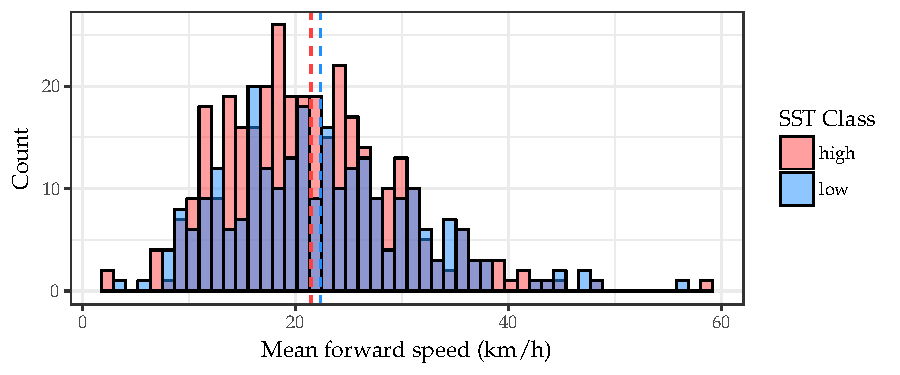
\includegraphics[width=0.9\textwidth]{images/natl-forward-speed}
	\caption{Mean forward speed histogram for the North Atlantic basin}
	\label{fig:natl-forward-speed}
\end{figure}

\begin{figure}[H]
	\centering
	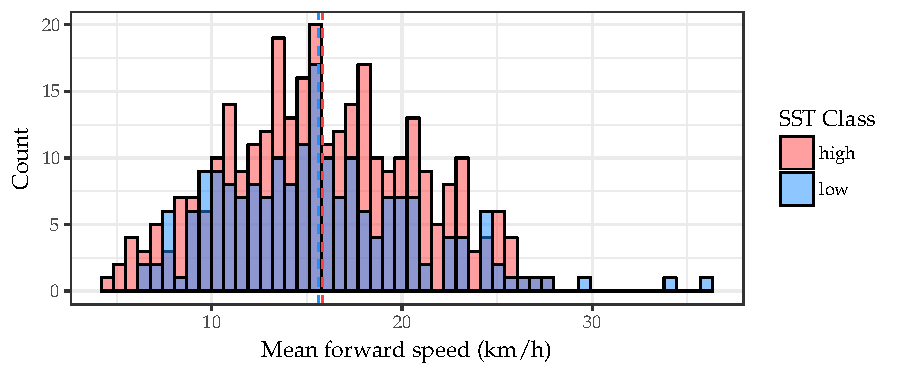
\includegraphics[width=0.8\textwidth]{images/epac-forward-speed}
	\caption{Mean forward speed histogram for the Northeast Pacific basin}
	\label{fig:epac-forward-speed}
\end{figure}
